\chapter{Experiments}
\label{sec:experiments}
This chapter starts with a proof of concept, showing that the principle of
O-MCTS and OL-MCTS works on a very simple game. Consequently, we will run O-MCTS
and OL-MCTS on a set of twenty-eight different games from the VGDL framework and
compare them to MCTS's perfomance.  These games include all games from the first
four training sets of the GVGAI competition, excluding puzzle games that can be
solved by a simple exhaustive search and have no random component (like NPCs,
for example). Each game consists of 5 levels. Firstly, we will compare O-MCTS's
performance to that of MCTS, by showing the win ratio and mean score of both
algorithms on all the games.  Secondly we show the improvement that OL-MCTS can
make on the games if it is allowed 4 games of learning time, and show the
progress it makes over 5 games.  Lastly we compare the three algorithms by
summing over all the games.  The goal of the algorithms is to primarily win as
many games as possible, while secondly maximizing the score. 

For these experiments we construct an option set which is aimed at providing
action sequences for any type of game, since the aim here is general video game
playing. Note that a more specific set of options can be created when the
algorithm should be tailored to only one type of games and similarly, more
options can be added to the algorithm easily.

\begin{itemize}[noitemsep]
	\item \texttt{ActionOption} executes a specific action once and then
		stops.
	\item \texttt{AvoidNearestNpcOption} makes the agent avoid the nearest NPC
	\item \texttt{GoNearMovableOption} makes the agent walk towards a
		movable game sprite (defined as movable by the VGDL) and stops when it
		is within a certain range of the movable
	\item \texttt{GoToMovableOption} makes the agent walk towards a
		movable until its location is the same as that of the movable
	\item \texttt{GoToNearestSpriteOfType} makes the agent walk to the nearest sprite of
		a specific type
	\item \texttt{GoToPositionOption} makes the agent walk to a specific position
	\item \texttt{WaitAndShootOption} waits until an NPC is in a specific location and
		then uses its weapon.
\end{itemize}

For each option type, a subtype per visible sprite type is created during the
game. For each sprite, an option instance of its corresponding subtype is
created. For example, the game \textit{zelda}, as seen in Figure \ref{fig:zelda},
contains three different sprite types (excluding the avatar and walls);
monsters, a key and a portal. The first level contains three monsters, one key
and one portal, and the aim of the game is to collect the key and walk towards
the portal without walking into the monsters. The score is increased by 1 if a
monster is killed (i.e., its sprite is on the same location as the sword sprite)
if the key is picked up, and when the game is won. \texttt{GoToMovableOption} and
\texttt{GoNearMovableOptions} are created for each of the three monsters and
for the key. A \texttt{GoToPositionOption} is created for the portal.  One
\texttt{GoToNearestSpriteOfType} is created per sprite type. One
\texttt{WaitAndShootOption} is created for the monsters, and one
\texttt{AvoidNearestNpcOption} is created. This set of options is $O$ in
Algorithms \ref{alg:omcts} and \ref{alg:olmcts}. In a state where, for example,
all the monsters are dead, the possible option set $\mathbf{p}_s$ does not
contain the \texttt{AvoidNearestNpcOption} and \texttt{GoToMovableOption}s and
\texttt{GoNearMovableOption}s for the monsters.

The \texttt{GoTo\ldots} options all utilize an adaptation of the A Star
algorithm to plan routes. An adaptation is needed, because at the beginning of
the game there is no knowledge of which sprites are traversable and which are
not. Thus, during every move that is simulated by the agent, the A Star module
has to update its beliefs about the location of walls and other blocking
objects. This is accomplished by comparing the movement the avatar wanted to
make to the movement that was actually made in game. If the avatar did not move,
it is assumed that all the sprites on the location the avatar should have
arrived in are blocking sprites. A Star keeps a \emph{wall score} for each
sprite type. When a sprite blocks the avatar, its wall score is increased by
one. Additionally, when a sprite kills the avatar, its wall score is increased
by 100, in order to prevent the avatar from walking into killing sprites.
Traditionally the A Star's heuristic uses the distance between two points. Our A
Star adaptation adds the wall score of the goal location to this heuristic,
encouraging the algorithm to take paths with a lower wall score. This method
enables A Star to try to traverse paths that were unavailable earlier, while
preferring safe and easily traversable paths. For example in \textit{zelda}, a
door is closed until a key is picked up. Our A Star version will still be able
to plan a path to the door once the key is picked up, winning the game.

We empirically optimize the parameters of the O(L)-MCTS algorithm
for these experiments. We use discount factor $\gamma = 0.9$, maximum action
time $t = 40$ milliseconds. The maximum search depth $d$ is set to 70, which is
higher than most alternative tree search algorithms, for example in the GVGAI
competition, use. The number of node visits after which \textsf{uct} is used,
$v$, is set to 40. Crazy stone parameter $K$ is set to $0.5$.  For comparison,
we use the MCTS algorithm provided with the Java implementation of VGDL with its
default value of maximum search depth of 10. Both algorithms have \textsf{uct}
constant $C_p = \sqrt{2}$. Unfortunately, comparing to Q-learning with options
was impossible, because the state space of these games is too big for the
algorithm to learn any reasonable behavior. All the experiments are run on an
Intel %\textsuperscript{\textregistered} 
Core %\texttrademark 
i7-2600, 3.40GHz quad core processor with 6 GB of DDR3, 1333 MHz RAM memory. For
all experiments, each algorithm plays each of the 5 levels of each game 20
times. 

\section{Toy Problem}

\lstinputlisting[caption=prey.txt, label=lst:preytxt, float=t]{../examples/gridphysics/prey.txt}

\lstinputlisting[caption=prey\_lvl0.txt, label=lst:preylvl, float=t]{../examples/gridphysics/prey_lvl0.txt}

For testing the performance of the algorithms, we create a simple test game. The
game aims to be simple to understand and easy to win, but it should be possible
to see any improvement an algorithm could achieve as well. We chose the
\emph{predator \& prey} game, in which the player is a predator, that should
catch its prey (an NPC) by walking into it. We decided to have three types of
prey, one that never moves, one that moves once in 10 turns and one that moves
once in 2 turns. This section describes how the game is made in VGDL.

As explained in chapter \ref{subsec:vgdl}, the first file that is needed by the
VGDL is the game description, which describes the game sprites and how they
interact with each other. The game description is shown in listing
\ref{lst:preytxt}.

Lines 2 to 8 describe the available sprites. There are two sprites in the game,
which are both \texttt{movable}: the avatar (predator) and the monster (prey).
The avatar is of type \texttt{MovingAvatar}, which means that the player has
four possible actions (up, right, down, left). The prey has three
instantiations, all of the type \texttt{RandomNPC}, which is an NPC that moves
about in random directions: the \texttt{inactivePrey}, which only moves every
3000 steps (which is more than the timeout explained shortly, so it never
moves); the \texttt{slowPrey} which moves once every 10 steps, and the
\texttt{fastPrey} which moves once every 2 steps.  By default, the
\texttt{MovingAvatar} can move once in each time step.

Lines 10 to 14 describe the level mapping. These characters can be used in the
level description files, to show where the sprites spawn. 

In the interaction set, Line 17 means that if the prey walks into the avatar (or
vice versa) this will kill the prey, and the player will get a score increase of
one point. Line 18 dictates that no \texttt{movable} sprite can walk through
walls.

Lastly, in the termination set, line 21 shows that the player wins when there
are no more sprites of the type \texttt{prey}, and line 22 shows that the player
loses after 100 time steps.

Listing \ref{lst:preylvl} shows a very simple level description. This level is
surrounded with walls and contains one avatar and one slow prey. 

The game can be used to test the functionality of an algorithm. The first level
is very simple and is only lost when the agent is not able to find the prey
within the time limit of 100 time steps, which is unlikely. A learning
algorithm should, however be able to improve the number of time steps it needs
to find the prey. The minimum number of time steps to win the game in level 1,
taking the optimal route, is six.

\section{Game Test Set}
\label{subsec:games}
The algorithms we propose are tested on a subset of the first four training sets
of the GVGAI competition. We exclude puzzle games that can be solved by an
exhaustive search, because these have no random components, and the algorithms
would not be able to benefit from the option set that was constructed for these
experiments. This leaves us with the twenty-eight games that are described in this
section. All games are lost when they take longer than 2000 time steps, unless
specified otherwise.

\begin{enumerate}
	\item Surround: 
		The aim of the game is to walk as far as possible. You get a point for
		every move you are able to make and afterwards, a non-traversable sprite
		is added in your previous location. The game is ended, and won, by using
		the \texttt{use} action. An NPC is doing the same as you and kills you
		on contact.
	\item Infection:
		The aim of the game is to infect as many healthy (green) animals (NPCs)
		as possible, by colliding with a bug or infected animal first, and then
		with a healthy animal. When animals collide with other infected animals,
		they get infected as well. Blue sprites are medics that cure infected
		animals and the avatar, but can be killed with the avatar's sword. The
		player wins when every animal is infected.
	\item Butterflies: 
		The avatar hunts butterflies, the avatar wins if he has caught (walked
		into) all of them. Butterflies spawn at certain locations, so sometimes
		waiting longer to end the game can increase the eventual score.
	\item Missile Command: 
		Missiles move towards some city-sprites that need to be defended by the
		avatar. The avatar can destroy missiles before they reach the city by
		standing next to a missile and using his weapon. When all missiles are
		gone and some of the city sprites are still left, the game is won. If
		all the city sprites are gone, the game is lost.
	\item Whackamole:
		The avatar must collect moles that appear at holes. The enemy player is
		doing the same. The player wins after 500 time steps and loses when it
		collides with the enemy.
	\item Aliens:
		Based on the commonly known game \textit{space invaders}. Aliens appear
		at the top of the screen. The avatar can move left or right and shoot
		missiles at them. The avatar loses when the aliens reach the bottom and
		wins when all the aliens are dead. The avatar should evade the aliens'
		missiles as well.
	\item Plaque attack:
		Hamburgers and hotdogs attack the teeth at the bottom of the screen. The
		avatar must shoot them with a projectile weapon in order to save at
		least one tooth. The avatar can repair damaged teeth by walking into
		them. The game is won if all the food is gone and lost if the teeth are
		gone.
	\item Plants:
		Emulating the \textit{Plants vs. Zombies} game, the avatar should plant
		plants that shoot peas at incoming zombies. The zombies can kill the
		plants by shooting back. The avatar wins when the time runs out, but
		loses when a zombie reaches the avatar's defensive field.
	\item Bait: 
		The avatar should collect a key and walk towards a goal. Holes in the
		ground kill the avatar when he moves into them, but can be closed by
		pushing boxes into them (after which both the hole and the box
		disappear). By collecting mushrooms, the player can get more points.
	\item Camel Race:
		The avatar must get to the finish line before any other camel does.
	\item Survive Zombies:
		The avatar should evade the zombies that walk towards him. When a zombie
		touches honey, it dies. If the avatar survives for 1000 time steps, it
		wins the game.
	\item Seaquest:
		The avatar can be killed by animals, or kill them by shooting them. The
		aim is to  rescue divers by taking them to the surface. The avatar can
		run out of oxygen, so it must return to the surface every now and then.
		The game is won after 1000 time steps, or lost if the avatar dies.
	\item Jaws:
		The avatar must shoot dangerous fish to collect the resources they drop.
		A shark appears at a random point in time, that can not be killed by
		shooting, but can be killed by touch, given that the avatar has enough
		resources. If he has too little resources, the game is lost. Otherwise,
		after 1000 time steps, the game is won.
	\item Firestorms:
		The avatar must avoid flames while traversing towards the exit. He can
		collect water, in order to survive hits by flames, but the game is lost
		if a flame hits the avatar when he has no water. 
	\item Lemmings:
		Lemmings are spawned from a door and try to get tot the exit. The avatar
		must destroy their obstacles. There are traps that have to be evaded by
		the avatar and the lemmings. The game is won when all the lemmings are
		gone, or lost when the avatar dies.
	\item Firecaster:
		The avatar must burn wooden boxes that obstruct his path to the exit.
		The avatar needs to collect ammunition in order to be able to shoot.
		Flames spread, being able to destroy more than one box, but the avatar
		should evade them as well. When the player's health reaches 0, he loses,
		but when he reaches the exit, he wins.
	\item Pacman:
		The avatar must clear the maze by eating all the dots, fruit pieces and
		power pills.  When the player collides with a ghost, it kills the
		avatar, unless he has eaten a power pill recently.
	\item Overload:
		The avatar must collect a determined number of coins before he is
		allowed to enter the exit. If the avatar collects more coins than that,
		he is trapped, but can kill marsh sprites with his sword for points.
	\item Boulderdash:
		The player collects diamons while digging through a cave. He should
		avoid boulders that fall from above, and avoid or kill monsters. If the
		avatar has enough diamonds, he may enter the exit and wins.
	\item Zelda:
		The avatar should collect a key and walk towards the door in order to
		win. He can kill monsters with his sword for additional points.
	\item Chase:
		The avatar chases and kills goats that are scared. However, when a
		scared ghost walks into the carcass of one of the others, he becomes
		angry, and can kill the avatar. When there are no scared goats left, the
		avatar wins.
	\item Digdug:
		The aim of the game is to collect all the gems and gold coins by digging
		a way through a cave. Enemies kill the players on collision. When the
		avatar presses \textsc{use} in two consecutive time steps, it shoots a boulder to
		kill the enemy.
	\item Bolo Adventures:
		The avatar should reach the goal. He can push around boxes 1 cell at a
		time, or boulders that roll until they hit another obstacle. Boulders
		can fill holes that obstruct the player's movement, and both boulders
		and boxes can block laser beams that kill the avatar.
	\item Roguelike:
		The avatar should escape a maze through the door. There are monsters
		that can be killed with a sword, after it has been picked up. Doors can
		be opened with keys. Extra points are awarded for picking up gold and
		gems. After being hit by an enemy, it is possible to exchange gold for
		health.
	\item Boulderchase:
		Similar to \textit{boulderdash}, but when an enemy is killed, it drops a
		diamond. Furthermore, in \textit{boulderdash} the enemy cannot dig
		routes through the environment, but here it can.
	\item Eggomania:
		A chicken at the top of the screen throws eggs. The aim of the game is
		to move from left to right in order to catch the eggs. If the avatar
		fails to catch even one, the game is lost. When the avatar
		has collected enough eggs, it is possible to shoot the chicken to win
		the game.
	\item Portals:
		The avatar needs to find the exit of the maze. He can use the available
		portals to teleport from one place to another. The aim of the game is to
		find the correct sequence of portals that lead to the exit. There are
		moving objects that kill the player on touch.
	\item Frogs:
		Like the commonly known game \textit{frogger}, the avatar is a frog,
		that needs to cross a busy road and a river. On the road, the frog
		should evade the trucks that move by. On the river, the frog should leap
		from tree trunk to tree trunk in order to reach the exit.
\end{enumerate}




\section{SMDP Q-learning}
\begin{figure}
	\centering
	\subfigure[Win ratio on \textit{prey}]{
		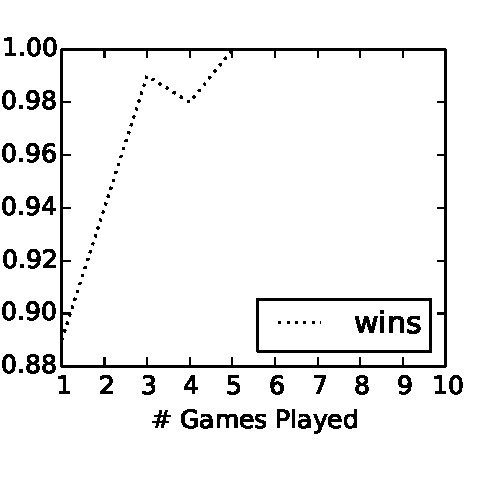
\includegraphics[scale=.48]{includes/winsQlearningPrey}
		\label{fig:wins-qlearning-prey}
	}
	\subfigure[Time taken for \textit{prey}]{
		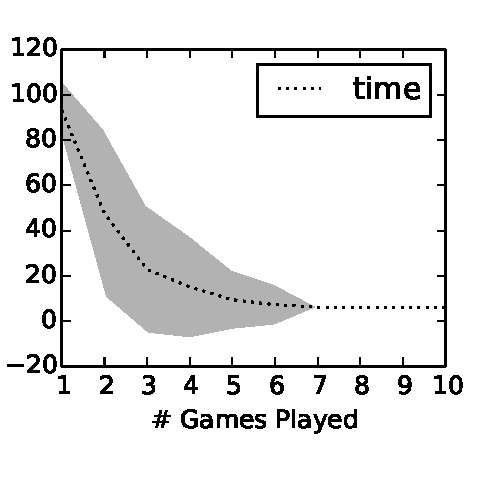
\includegraphics[scale=.48]{includes/timeQlearningPrey}
		\label{fig:time-qlearning-prey}
	}
	\caption{Performance of SMDP Q-learning on the toy problem.}
	\label{fig:qlearning}
\end{figure}

Firstly, we will test our implementation of SMDP Q-learning. This section shows
the results on the toy problem \textit{prey} and a set of the other test games.

In order to get SMDP Q-learning to work correctly, we need to serialize the
state space. Furthermore, to prevent the Q-table to become too big, we apply a
state space reduction. These are the values that are saved:

\begin{itemize}
	\item The avatar orientation
	\item The avatar's resources (this is often a number, for example
		\texttt{"diamonds:3"})
	\item The Euclidean distance and direction to the nearest of:
		\begin{itemize}
			\item NPCs
			\item Other Movable sprites
			\item Resources
			\item Portals
			\item Other immovable sprites
		\end{itemize}
\end{itemize}

This crude state space reduction removes information about the map and location
of the avatar, but enables the algorithm to keep a smaller Q-table, enabling it
to work on more games, without running out of memory.

In the first experiment, we check if SMDP Q-learning, with our option set and
state space reduction, works by applying it to the test game. The results can be
seen in figure \ref{fig:qlearning}. We can see that the algorithm wins
consistently starting at game 3 and that the time it takes to win quickly and
almost always converges to 6, the least number of steps possible to win the
game. After that, it wins consistently by applying the correct options. This
indicates that the values for the Q-table converge correctly.

Secondly, we run the algorithm on all the games described in chapter  
\ref{subsec:games}. 

\section{O-MCTS}
\label{subsec:omcts}
\begin{figure}
	\centering
	\makebox[\columnwidth]{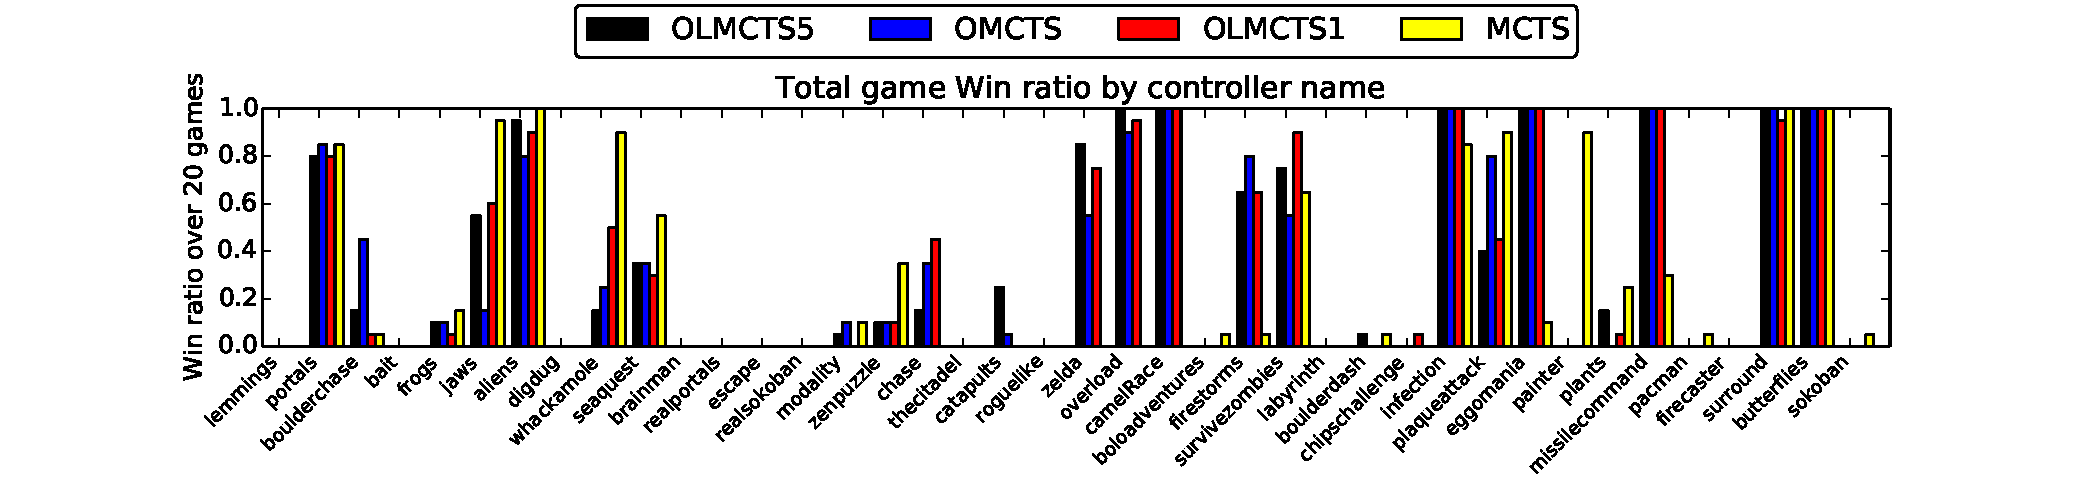
\includegraphics[width=1.25\textwidth]{includes/wins}}
	\vspace{-.8cm}
	\caption{Win ratio of the algorithms per game on all levels.}
	\label{fig:wins}
	\centering
	\makebox[\columnwidth]{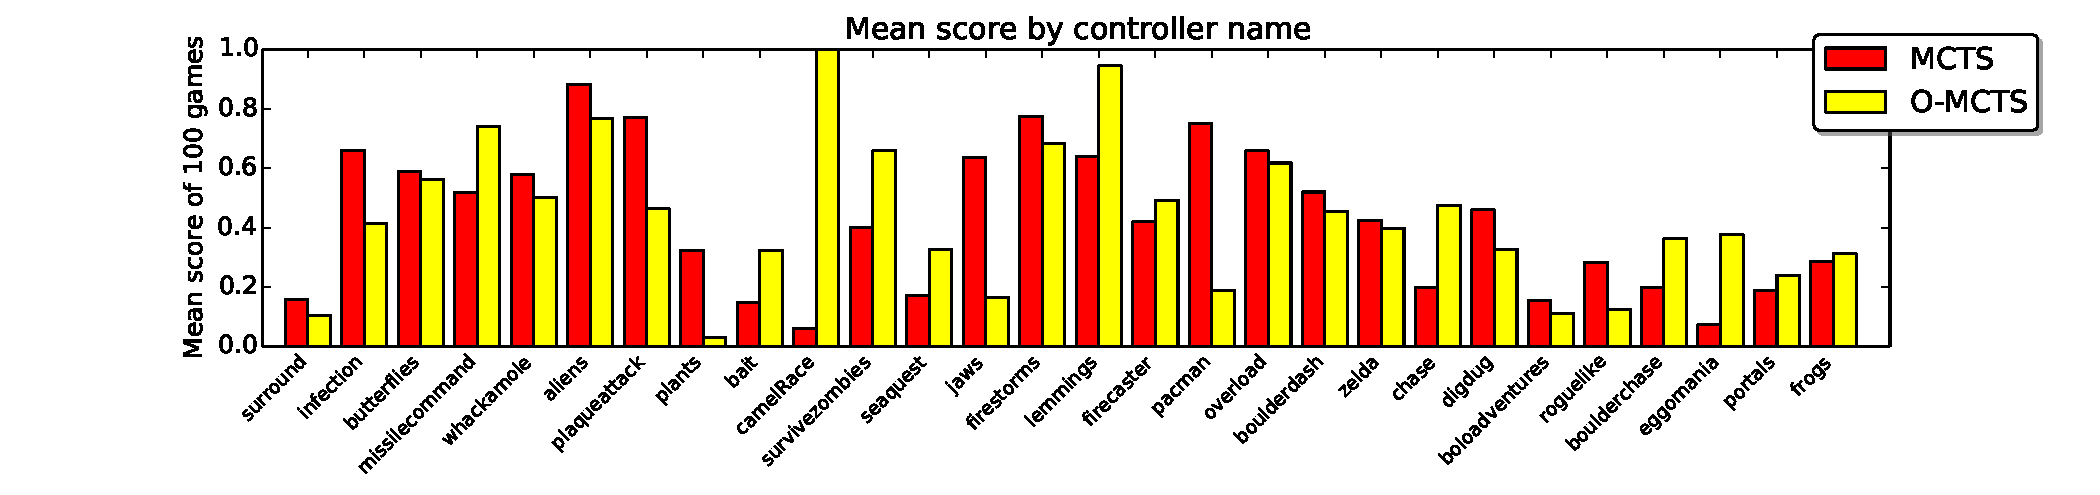
\includegraphics[width=1.25\textwidth]{includes/scores}}
	\vspace{-.8cm}
	\caption{Mean normalized score of the algorithms per game 1 means the
	highest score achieved by all the algoriths, 0 the lowest.}
	\label{fig:scores}
\end{figure}

In the first experiment, we compare O-MCTS and MCTS. Figures \ref{fig:wins} and
\ref{fig:scores} respectively show the win ratio and normalized score of the
algorithms for each game. The games are ordered by the performance an algorithm
that always chooses a random action, indicating the complexity of the games.
From left to right, the random algorithm's win ratio and score decreases. As can
be seen in Figure \ref{fig:wins}, the O-MCTS algorithms performs at least as
good as MCTS in almost all games. 

O-MCTS greatly outperforms MCTS in the games \textit{missile
command}, \textit{overload}, \textit{firestorms}, \textit{boulderchase},
\textit{zelda}, \textit{bait}, \textit{camel race}, \textit{eggomania},
\textit{firecaster}, \textit{chase} and \textit{lemmings}, winning many more
games. Analyzing the algorithm's actions for these games, we can see that
the algorithm succeeds in efficiently planning paths in a dangerous environment,
enabling it to do a further forward search than the ordinary Monte Carlo tree
search. \textit{Camel race} requires the player to move to the right for 80
consecutive turns, which is very hard for MCTS, since it only looks forward 10 
turns. O-MCTS almost always wins, since it can plan forward a lot further. In
Overload, a sword has to be picked up before the avatar can finish the game,
which seems to be too hard for MCTS, but poses less of a problem for O-MCTS.
Furthermore, in Zelda we can see that the MCTS algorithm achieves roughly the
same score as O-MCTS, but does not win the game, since picking up the key and
walking towards the door is a difficult action sequence. We assume that the
score achieved by MCTS is because it succeeds in killing the monsters, whereas
O-MCTS achieves its score by picking up the key and walking to the door.  These
results indicate that O-MCTS performs better than MCTS in games where a longer
sequence of action planning has to be done.

The MCTS algorithm performs significantly better than O-MCTS in
\textit{whackamole}, \textit{jaws}, \textit{seaquest} and \textit{plaque
attack}. The similarity of these games is that they have a very big number of
different sprites, for each of which several options have to be created by
O-MCTS.  When the number of options becomes too big, constructing the set of
possible options $\mathbf{p}_s$ for every state $s$ becomes so time-consuming
that the algorithm has too little time to build a tree and find the best
possible action. In another experiment, we increased the computation time for
O-MCTS to 120ms and found that the win ratio of O-MCTS increases to around $0.8$
for \textit{seaquest} and \textit{plaque attack}.
% TODO: I probably want to check if MCTS's performance also increases with more
% computation time

\begin{figure}
	\centering
	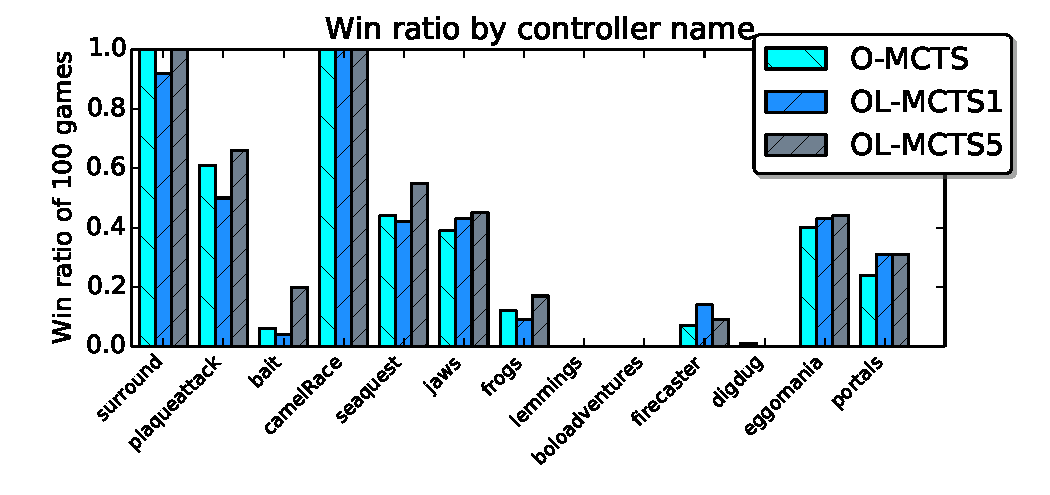
\includegraphics[width=\columnwidth]{includes/winsOLMCTS}
	\vspace{-.8cm}
	\caption{Win ratio comparison of OL-MCTS and O-MCTS.}
	\label{fig:wins-olmcts}
\end{figure}

\begin{figure}
	\centering
	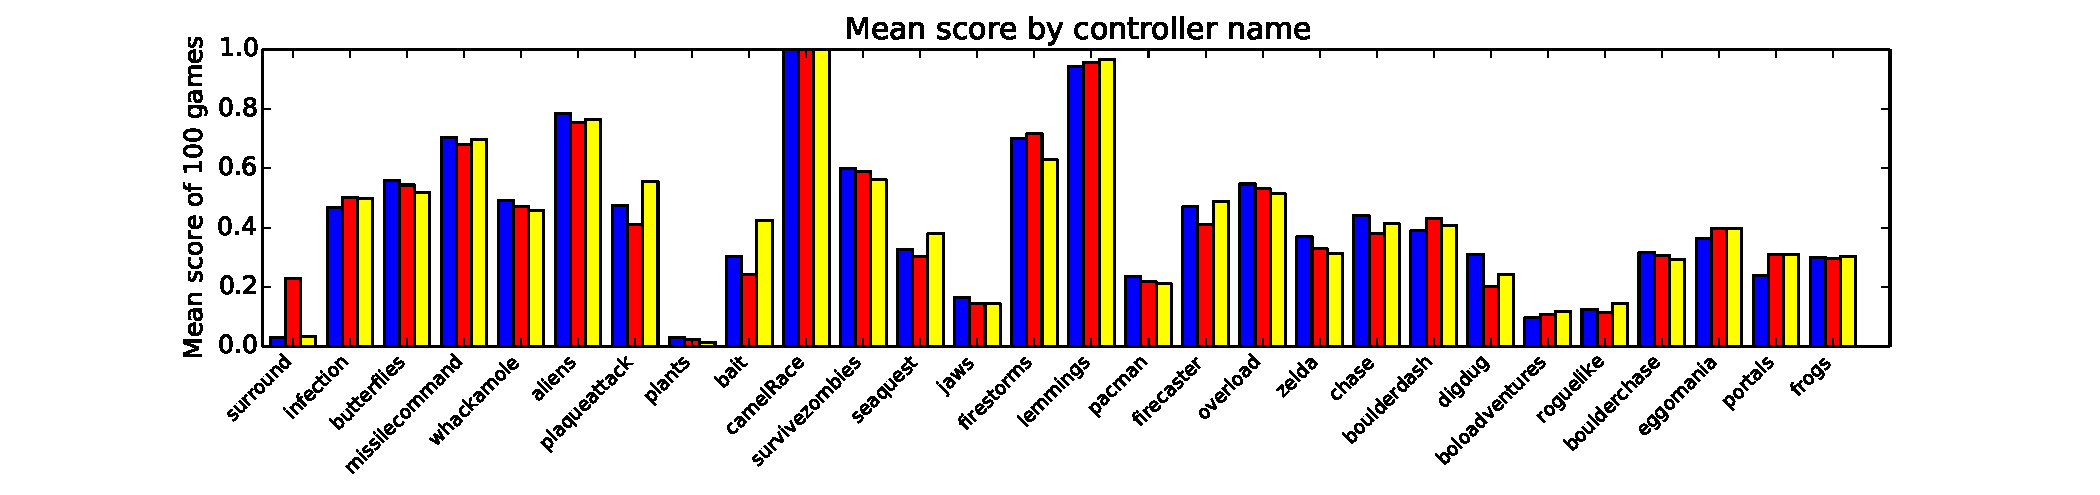
\includegraphics[width=\columnwidth]{includes/scoresOLMCTS}
	\vspace{-.8cm}
	\caption{Normalized score comparison of OL-MCTS and O-MCTS.}
	\label{fig:scores-olmcts}
\end{figure}

\section{OL-MCTS}
\label{subsec:olmcts}
For the second experiment, we compare OL-MCTS to O-MCTS, by running it on the
same set of games. The option learning algorithm is allowed four learning games,
after which the fifth is used for the comparisons. Figures \ref{fig:wins-olmcts}
and \ref{fig:scores-olmcts} show the games for which the results of OL-MCTS
differ from O-MCTS. For the other games, the performance was approximately the
same. Here OL-MCTS1 shows the performance of OL-MCTS on the first game. OL-MCTS5
shows the performance of the algorithm after learning for four games. 

We can see that, although the first iteration of OL-MCTS sometimes performs a
bit worse than O-MCTS, the fifth iteration often scores at least as high, or
higher than O-MCTS. We expect that the loss of performance in OL-MCTS1 is
because of the overhead that is created by the crazy stone algorithm: A sorting
of all the options has to take place in each game state. The learning algorithm
significantly improves score and win ratio for the game \textit{bait}, which is
a game in which the objective is to reach a goal portal after collecting a key.
The player can push boxes around to open paths. There are holes in the ground
that kill the player, unless they are filled with boxes, which make both the
hole and the box disappear. Figure \ref{fig:learning-results} shows the
improvement in score and win ratio for this game. There are two likely 
explanations for this improvement: 1.) There are sprites that kill the player,
which are evaded by the algorithm when it has learned to do so.  2.) The
algorithm learns that it should pick up the key.

\begin{figure}
	\centering
	%\subfigure[Learning \textit{bait}]{
	%	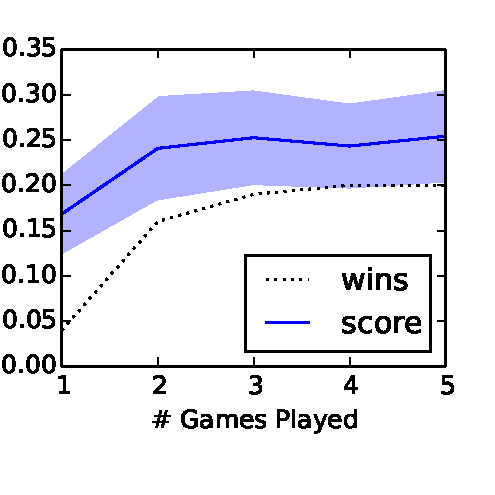
\includegraphics[scale=.44]{includes/learning}
	%	\label{fig:learning-results}
	%}
	%\subfigure[Totals]{
	%	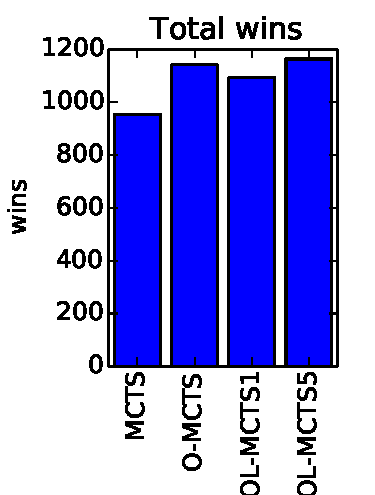
\includegraphics[scale=.44]{includes/totals.pdf}
	%	\label{fig:total-results}
	%}
	\caption{Learning improvement on game \textit{bait}, it shows win ratio and
		normalized score. Total number of wins of the algorithms on
	all games.}
\end{figure}

\section{Totals}
\label{subsec:totals}
Figure \ref{fig:total-results} shows the sum of wins over all games, all levels.
It shows a significant ($p < 0.05$) improvement of O-MCTS and OL-MCTS over MCTS.
There is no significant difference in performance of OL-MCTS over O-MCTS,
although our results indicate that it does improve for some of the games.

Summarizing, our tests indicate that on complex games O-MCTS outperforms MCTS.
For other games it performs at least as well, as long as the number of game
sprites is not too high. 
%TODO: How many sprites?
The OL-MCTS algorithm performs worse than O-MCTS before learning, on some of the
games, like \textit{surround}, \textit{plaqueattack}, and \textit{bait}, but
can, for some of the games, increase performance significantly.
